% Quiver visualization of the 1-form dz (full-arrow form) on the complex plane:
% at each grid point, short arrows in the four axis directions are
% labeled with the value of the form on that tangent vector.
% Source: book/tex/riemann-surface/forms.tex (generated; edit the
% generator comment in the repo history rather than by hand).
\documentclass[border=2mm]{standalone}
\usepackage{tikz}
\usepackage{amsmath}
\begin{document}
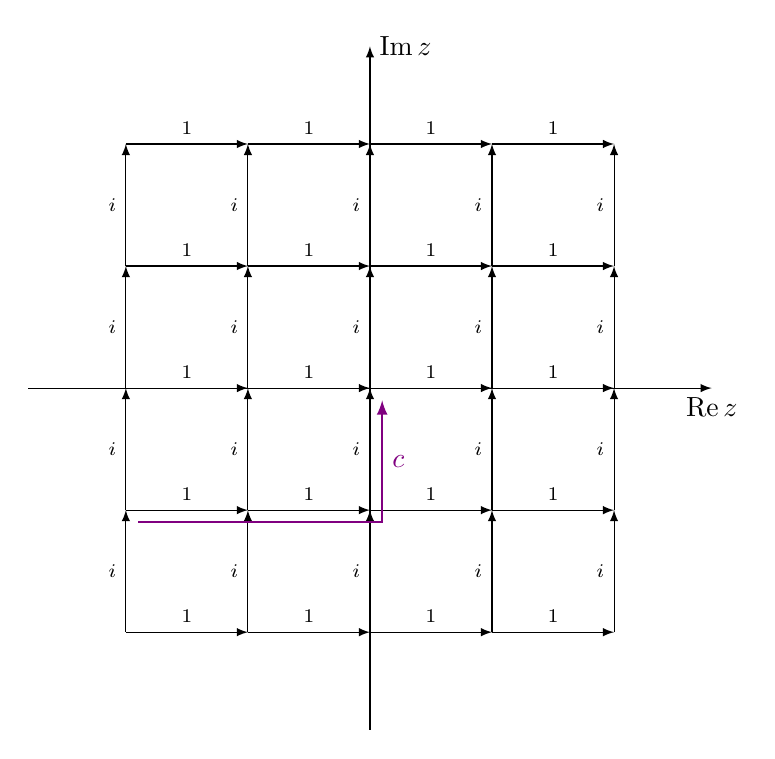
\begin{tikzpicture}[scale=1.55,>=latex]
  \draw[->] (-2.8,0) -- (2.8,0) node[below] {$\operatorname{Re} z$};
  \draw[->] (0,-2.8) -- (0,2.8) node[right] {$\operatorname{Im} z$};
  \draw[->] (-2,-2) -- (-1,-2) node[midway, above] {\scriptsize $1$};
  \draw[->] (-2,-2) -- (-2,-1) node[midway, left] {\scriptsize $i$};
  \draw[->] (-2,-1) -- (-1,-1) node[midway, above] {\scriptsize $1$};
  \draw[->] (-2,-1) -- (-2,0) node[midway, left] {\scriptsize $i$};
  \draw[->] (-2,0) -- (-1,0) node[midway, above] {\scriptsize $1$};
  \draw[->] (-2,0) -- (-2,1) node[midway, left] {\scriptsize $i$};
  \draw[->] (-2,1) -- (-1,1) node[midway, above] {\scriptsize $1$};
  \draw[->] (-2,1) -- (-2,2) node[midway, left] {\scriptsize $i$};
  \draw[->] (-2,2) -- (-1,2) node[midway, above] {\scriptsize $1$};
  \draw[->] (-1,-2) -- (0,-2) node[midway, above] {\scriptsize $1$};
  \draw[->] (-1,-2) -- (-1,-1) node[midway, left] {\scriptsize $i$};
  \draw[->] (-1,-1) -- (0,-1) node[midway, above] {\scriptsize $1$};
  \draw[->] (-1,-1) -- (-1,0) node[midway, left] {\scriptsize $i$};
  \draw[->] (-1,0) -- (0,0) node[midway, above] {\scriptsize $1$};
  \draw[->] (-1,0) -- (-1,1) node[midway, left] {\scriptsize $i$};
  \draw[->] (-1,1) -- (0,1) node[midway, above] {\scriptsize $1$};
  \draw[->] (-1,1) -- (-1,2) node[midway, left] {\scriptsize $i$};
  \draw[->] (-1,2) -- (0,2) node[midway, above] {\scriptsize $1$};
  \draw[->] (0,-2) -- (1,-2) node[midway, above] {\scriptsize $1$};
  \draw[->] (0,-2) -- (0,-1) node[midway, left] {\scriptsize $i$};
  \draw[->] (0,-1) -- (1,-1) node[midway, above] {\scriptsize $1$};
  \draw[->] (0,-1) -- (0,0) node[midway, left] {\scriptsize $i$};
  \draw[->] (0,0) -- (1,0) node[midway, above] {\scriptsize $1$};
  \draw[->] (0,0) -- (0,1) node[midway, left] {\scriptsize $i$};
  \draw[->] (0,1) -- (1,1) node[midway, above] {\scriptsize $1$};
  \draw[->] (0,1) -- (0,2) node[midway, left] {\scriptsize $i$};
  \draw[->] (0,2) -- (1,2) node[midway, above] {\scriptsize $1$};
  \draw[->] (1,-2) -- (2,-2) node[midway, above] {\scriptsize $1$};
  \draw[->] (1,-2) -- (1,-1) node[midway, left] {\scriptsize $i$};
  \draw[->] (1,-1) -- (2,-1) node[midway, above] {\scriptsize $1$};
  \draw[->] (1,-1) -- (1,0) node[midway, left] {\scriptsize $i$};
  \draw[->] (1,0) -- (2,0) node[midway, above] {\scriptsize $1$};
  \draw[->] (1,0) -- (1,1) node[midway, left] {\scriptsize $i$};
  \draw[->] (1,1) -- (2,1) node[midway, above] {\scriptsize $1$};
  \draw[->] (1,1) -- (1,2) node[midway, left] {\scriptsize $i$};
  \draw[->] (1,2) -- (2,2) node[midway, above] {\scriptsize $1$};
  \draw[->] (2,-2) -- (2,-1) node[midway, left] {\scriptsize $i$};
  \draw[->] (2,-1) -- (2,0) node[midway, left] {\scriptsize $i$};
  \draw[->] (2,0) -- (2,1) node[midway, left] {\scriptsize $i$};
  \draw[->] (2,1) -- (2,2) node[midway, left] {\scriptsize $i$};
  \draw[->, thick, violet] (-1.9,-1.1) -- (0.1,-1.1) -- (0.1,-0.1) node[midway, right] {$c$};
\end{tikzpicture}
\end{document}
